\documentclass[11pt]{article}
\usepackage[T1]{fontenc}
\usepackage[sfdefault]{FiraSans}
\usepackage[a4paper, left=2cm, right=2cm, top=2.5cm, bottom=2.5cm]{geometry}
\usepackage{hyperref}
\usepackage{graphicx}
\usepackage{enumitem}
\usepackage{titling}
\usepackage{adjustbox}
\usepackage{xcolor}
\usepackage{titlesec}
\usepackage[utf8]{inputenc}
\usepackage{wrapfig}
\usepackage{babel}
\usepackage{tcolorbox}
\usepackage{fancyhdr}
\usepackage{caption}
\usepackage{subcaption}
\usepackage{xr}
\usepackage{ulem}
\usepackage{lastpage}
\usepackage{csquotes}
\usepackage{tabularx}
\usepackage{minted}
\usepackage{tikz}
\usepackage{pgfplots}
\usepackage{array}
\usepackage{multirow}
\usepackage{standalone}
\usepackage{footmisc}
\usepackage{multicol}
\usepackage{import}
\usepackage{MnSymbol}
\usepackage{hyperref}
\usepackage{newunicodechar}
\usepackage[all]{nowidow}
\usepackage[acronym, toc]{glossaries}
\usepackage[nottoc]{tocbibind}

\hypersetup{
    colorlinks,
    linkcolor={blue!45!black},
    citecolor={blue!50!black},
    urlcolor={blue!80!black}
}

\def\UrlBreaks{\do\/\do-\do_}

\def\semester{2024}
\def\program{Master Data Science}
\def\course{Data Intensive Computing}
\def\coursefull{Data Intensive Computing}
\def\assigmentlong{Group 16: Exercise 1}
\def\assigment{Exercise I}
\def\studentlong{Arash Behaein - 12324255\\
                 Brais Guardado Collazo - 12233000\\
                 Dinesh Thakur - 12334943}
\def\student{A. Behaein, B. Guardado Collazo, D. Thakur}

\pagestyle{fancy}
\fancyhf{}
\setlength{\headsep}{1.2cm}


\lhead{
    \includegraphics[height=1cm]{logo.png}
}
\chead
{
     \assigmentlong
     }
\rhead
{
     \semester
}
\lfoot
{
    \student \\
    TU Wien - \program
}
\rfoot
{
            \thepage/\pageref{LastMainPage} \\
            \today
}

\begin{document}
\begin{titlepage}
    \vspace*{\fill}
    \centering
      \vspace{-9cm}

    \Huge{\textbf{\coursefull}}\\[1.5cm]
    \Large{\assigmentlong}\\[2cm]
    \large{\studentlong}\\
    \vfill
    \includegraphics[width=0.4\textwidth]{logo.png}

        \vspace{0.7cm}
    \large{Course: \course}\\
    \large{Academic Year: \semester}\\
    
    \large{\today}\\
\end{titlepage}

%%%%%%%%%%%%%%%%%%%%%%%%%%%%%%%%%%%%%%%%%%%%%%%%%%%%%%%%%%%%%%%%%%%%%%%%%%%%%%%%%%%%%%%%%%%%%%%% PAGE 2

\newpage
% \pagestyle{empty}
\tableofcontents
% \newpage 
\pagestyle{fancy}
\setcounter{page}{1}

\renewcommand{\abstractname}{Introduction}
\vskip1cm

\section{Introduction}

For this first assigment, we have been tasked with finding the most discriminative terms for each category on the \href{https://cseweb.ucsd.edu/~jmcauley/datasets/amazon/links.html}{Amazon Review Dataset 2014}, which consists of billions of reviews across 22 product categories. Identifying discriminative terms for each category is essential for text classification,  which involves categorizing text data based on its content. Some use cases of text  classification include sentiment analysis, spam detection, and topic modeling, among  others. To find the most discriminative terms, the chi-square metric applied to text processing will be used, which is a measure of the association between categorical variables.

Additionally, a key aspect of this job is performance, since to compute the chi-square value of a single word/category pair, the whole dataset must have been traversed first. This dataset precisely has an approximate size of 50GB, counting roughly 58 billion (billion $\equiv 10^9$) records. Clearly, an impossible task to accomplish if using \textit{traditional} computing methods.

This is where distributed computing comes into play. Using the MapReduce programming model, we can efficiently process large datasets across a distributed cluster. By dividing the workload into smaller tasks and distributing them across multiple nodes, MapReduce enables faster computation and better resource utilization.

The idea behind this paradigm is to bring the logic (the code) to the data, and not the other way around. MapReduce revolves around two core concepts: mapping and reducing (hence the name). The mapping phase is responsible for transforming the input data into a set of key-value pairs, which are then emitted through the network. An intermediate phase called shuffling takes place, where the key-value pairs are sorted and grouped by their key. These sorted key-value pairs are then passed to the reducing phase, which performs some user defined logic on the values associated with each key. The result of the reducer can now be the final output of the MapReduce job or serve as input to another MapReduce round.

\section{Problem Overview}

The chi-square metric has been mentioned as a measure of the association between categorical variables. But, it has not been properly defined in this context, text classification. The metric, computed for a term $t$ and a category $c$, is defined as:

$$
\chi^2_{tc} = \frac{N(AD - BC)^2}{(A + B)(A + C)(B + D)(C + D)}
$$
where:
\begin{itemize}
    \item $A$ is the number of documents in category $c$ that contain term $t$.
    \item $B$ is the number of documents not in category $c$ that contain term $t$.
    \item $C$ is the number of documents in category $c$ that do not contain term $t$.
    \item $D$ is the number of documents not in category $c$ that do not contain term $t$.
    \item $N$ is the total number of documents on the corpus.
\end{itemize}

Given this, the challenge of this assignment resides in finding a clever way of counting this A, B, C, and D values for each term and category pair using the MapReduce paradigm. The final output of the MapReduce job should be an ordered list of the top 75 terms for each category, based on their chi-square value.

Preprocessing the text data is also a crucial step in this process, since it can help aleviate the overall workload. The steps used in this assignment have been:

\begin{itemize}
    \item Tokenization: splitting the text into words.
    \item Lowercasing: converting all words to lowercase.
    \item Removing stopwords: removing common words that do not carry much meaning, such as \textit{the}, \textit{is}, \textit{and}, etc.
    \item Stemming: reducing words to their root form, such as \textit{running} to \textit{run}.
\end{itemize}

Important to note is that stemming was not a requirement for this task. Experiments with and without stemming revealed a better performance for MapReduce rounds which implemented stemming. For this reason alone, we have decided to leave stemming in the preprocessing pipeline, but the final decision of adding stemming or not has to be based on the true goal of the task, which is not clear from the assignment description (we were only tasked with finding the most discriminative terms for each category, \textit{but then what?}).

\section{Approach \& Methodology}

\begin{figure}
    \centering
    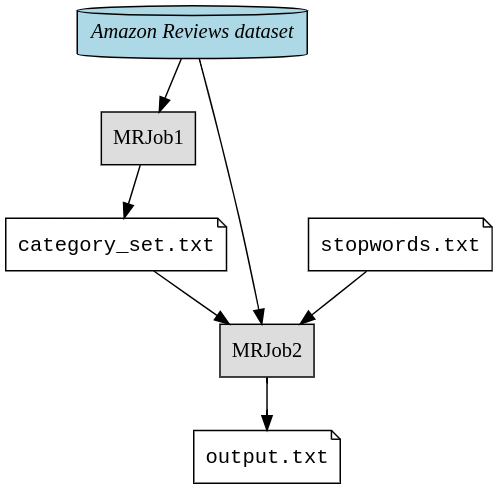
\includegraphics[width=0.55\linewidth]{img/highLevelPipe.png}
    \caption{High level pipeline overview}
    \label{fig:highLevelPipe}
\end{figure}

Let us first describe the overall idea of the implementation. We know the dataset is divided into several partitions, and during the mapping phase, each node will perform the same operations on the data available to it. There is no such thing as *shared memory*, each mapper works alone and does not have access to the data processed by other mappers. Therefore, our core idea has been to compute a \textit{local subset} of A, B, C, and D values for each term and category pair on every mapper, and then pass this information to the reducer. The reducer then aggregates the local counts for each category/term pair and computes its final chi-square value. The top 75 terms for each category are then emitted as the final output.

Let us now dive deeper. The overall work is divided into two MapReduce rounds. Important to note is that, even though they operate in series, the input of the second MapReduce step is not comprised only of the output of the first. This is illustrated in Figure \ref{fig:highLevelPipe}.



The first MapReduce (\verb|MRJob1| on the figure) step simply goes through the dataset and finds the set of categories. This set of categories will serve as an auxiliary input for the second MapReduce round, where the actual computation of the chi-square values takes place. A detailed view on the key value pairs used on \verb|MRJob1| is shown in Figure \ref{fig:categoryCounter}.

\begin{figure}
    \centering
    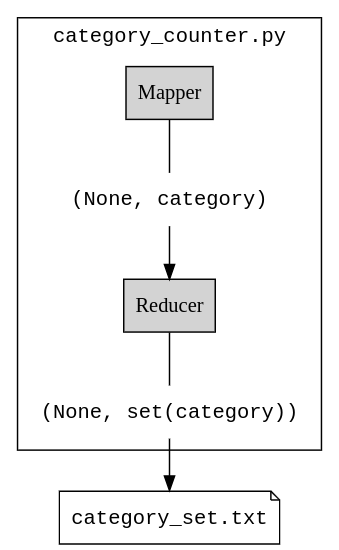
\includegraphics[width=0.35\linewidth]{img/categoryCounter.png}
    \caption{MRJob1}
    \label{fig:categoryCounter}
\end{figure}

The second MapReduce step \verb|MRJob2| does the heavy lifting. Making use of the \verb|*_init()| and \verb|*_final()| methods from \verb|mrjob|, we count one \verb|mapper_init()|, one \verb|mapper_final()| and then the standard \verb|mapper()|, \verb|combiner()| and \verb|reducer()| methods. A key aspect of using the \verb|mapper_init()| and \verb|mapper_final()| methods is that they are only called once per mapper, and allow to use shared memory between different mapper calls. With this we can first go through the whole partition on the mapper and store the preprocessed data on a Python container (a dictionary). Then, on \verb|mapper_final|, results are aggregated and yielded. This is illustrated in Figure \ref{fig:chiComputer}.

\begin{figure}
    \centering
    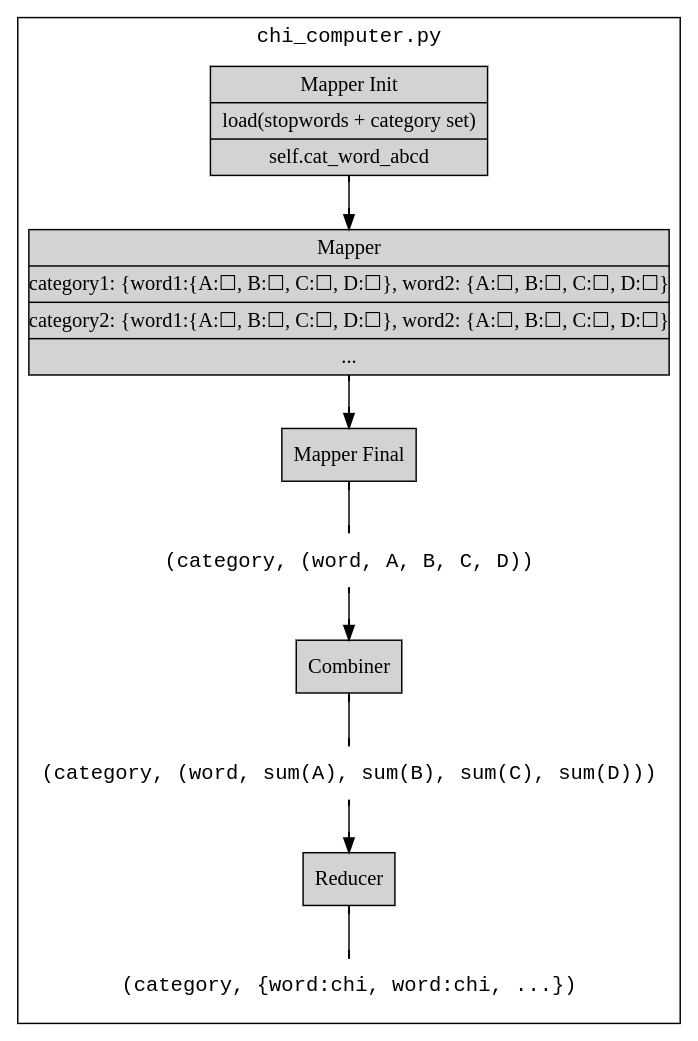
\includegraphics[width=0.75\linewidth]{img/chiComputer.png}
    \caption{MRJob2}
    \label{fig:chiComputer}
\end{figure}

The key emitted by the mapper is the category, and the value is a tuple of the form (term, A, B, C, D). Since the output of the mapper is still a local subset of the A, B, C, D values, the reducer first needs to aggregate these values for each category/term pair, and then compute the final chi-square value. As soon as this chi value is computed, it is pushed into a \verb|heapq| (\href{https://docs.python.org/3/library/heapq.html}{documentation}). This is a special Python container that keeps the elements ordered. Using it allows to solve two issues in one go. First, memory starvation: by forcing the length of the heap to be 75, we ensure the container size does not get out of hand and spills to hard memory. Secondly, by keeping a priority queue, we remove the need of sorting the final list of terms once finished.

\section{Results}

During development of this algorithm, a shorter version of the dataset was used, containing just 0.01\% of the original data. Output correctness of this smaller dataset could not be verified by \textit{official} means (\href{https://tuwel.tuwien.ac.at/mod/forum/discuss.php?d=423734}{TUWEL thread}), but comparing results with other groups' algorithms has increased confidence on the output's appropriateness. Regarding performance, 60 seconds have consistently been measured as the time needed to execute the second MapReduce step locally on the smaller dataset. Moving to the cluster, 120 seconds were consistently measured for the same MapReduce step. Experiments with the full dataset were not as thorough as with the smaller dataset, because performance turns out to be a catastrophe. Out of the few times the full dataset was run, the second MapReduce step took about 3 hours to complete. Efforts were made to optimize the code, but to no avail. We have been unable to explain or identify where the bottleneck is, since execution of the mapper for the development set takes most of the time, and the reducer is almost immediate. Moving on to the full dataset, the mapper takes only 12 minutes, and the reducer the remaining 3 hours. It is reasonable to assume that the bottleneck is in the reducer, but we have been unable to identify the cause.

Another point to which we would like to bring attention to is one outlier identified on the output. It is most likely due to some error on our preprocessing pipeline. It just appears on the category \verb|Apps_for_Android|, there is a term with 669.5 chi-square value. This term appears to be some escape sequence or similar, since it is rendered as "" on the output. We have been unable to remove it.

\section{Conclusion}

On this assignment we have implemented a MapReduce algorithm to find the most discriminative terms for each category on the Amazon Review Dataset 2014. Our approach has been to compute a local subset of the A, B, C, and D values for each term and category pair on the mapper, and then pass this information to the reducer. The algorithm has been tested on a smaller version of the dataset, and the results have been promising. However, performance on the full dataset has been a major issue, with the second MapReduce step taking about 3 hours to complete. Efforts to optimize the code have been unsuccessful, and the bottleneck has not been identified.

\label{LastMainPage}
\end{document}